% Options for packages loaded elsewhere
\PassOptionsToPackage{unicode}{hyperref}
\PassOptionsToPackage{hyphens}{url}
\PassOptionsToPackage{dvipsnames,svgnames*,x11names*}{xcolor}
%
\documentclass[
  11pt,
]{article}
\usepackage{lmodern}
\usepackage{amssymb,amsmath}
\usepackage{ifxetex,ifluatex}
\ifnum 0\ifxetex 1\fi\ifluatex 1\fi=0 % if pdftex
  \usepackage[T1]{fontenc}
  \usepackage[utf8]{inputenc}
  \usepackage{textcomp} % provide euro and other symbols
\else % if luatex or xetex
  \usepackage{unicode-math}
  \defaultfontfeatures{Scale=MatchLowercase}
  \defaultfontfeatures[\rmfamily]{Ligatures=TeX,Scale=1}
\fi
% Use upquote if available, for straight quotes in verbatim environments
\IfFileExists{upquote.sty}{\usepackage{upquote}}{}
\IfFileExists{microtype.sty}{% use microtype if available
  \usepackage[]{microtype}
  \UseMicrotypeSet[protrusion]{basicmath} % disable protrusion for tt fonts
}{}
\makeatletter
\@ifundefined{KOMAClassName}{% if non-KOMA class
  \IfFileExists{parskip.sty}{%
    \usepackage{parskip}
  }{% else
    \setlength{\parindent}{0pt}
    \setlength{\parskip}{6pt plus 2pt minus 1pt}}
}{% if KOMA class
  \KOMAoptions{parskip=half}}
\makeatother
\usepackage{xcolor}
\IfFileExists{xurl.sty}{\usepackage{xurl}}{} % add URL line breaks if available
\IfFileExists{bookmark.sty}{\usepackage{bookmark}}{
\usepackage{hyperref}
}
\hypersetup{
  pdftitle={Cours sur les tableaux},
  pdfauthor={Première NSI, Lycée du Parc},
  colorlinks=true,
  linkcolor=Maroon,
  filecolor=Maroon,
  citecolor=Blue,
  urlcolor=Blue,
  pdfcreator={LaTeX via pandoc}}
\urlstyle{same} % disable monospaced font for URLs
\usepackage[top=20mm,left=20mm,right=20mm,heightrounded]{geometry}
\usepackage{listings}
\newcommand{\passthrough}[1]{#1}
\lstset{defaultdialect=[5.3]Lua}
\lstset{defaultdialect=[x86masm]Assembler}
\usepackage{graphicx}
\makeatletter
\def\maxwidth{\ifdim\Gin@nat@width>\linewidth\linewidth\else\Gin@nat@width\fi}
\def\maxheight{\ifdim\Gin@nat@height>\textheight\textheight\else\Gin@nat@height\fi}
\makeatother
% Scale images if necessary, so that they will not overflow the page
% margins by default, and it is still possible to overwrite the defaults
% using explicit options in \includegraphics[width, height, ...]{}
\setkeys{Gin}{width=\maxwidth,height=\maxheight,keepaspectratio}
% Set default figure placement to htbp
\makeatletter
\def\fps@figure{htbp}
\makeatother
\setlength{\emergencystretch}{3em} % prevent overfull lines
\providecommand{\tightlist}{%
  \setlength{\itemsep}{0pt}\setlength{\parskip}{0pt}}
\setcounter{secnumdepth}{5}

\title{Cours sur les tableaux}
\usepackage{etoolbox}
\makeatletter
\providecommand{\subtitle}[1]{% add subtitle to \maketitle
  \apptocmd{\@title}{\par {\large #1 \par}}{}{}
}
\makeatother
\subtitle{Thème types construits}
\author{Première NSI, \href{https://frederic-junier.org/}{Lycée du
Parc}}
\date{}

%%%jolis boites

\usepackage{fancybox, graphicx}



%%%%%%%%%%%%%%%%Packages et Macros Frederic%%%%%%%%%%%%%%%%%%%%%%%%%%%%%


%%%%Insertion de liens hypertextes %%%%

            
%%%%%%%%%%PSTricks%%%%%%%%%%%%

\usepackage{pstricks,pst-plot,pst-text,pst-tree,pst-eps,pst-fill,pst-node,pst-math,pstricks-add,pst-xkey,pst-eucl}


%%%%%%%Tikz%%%%%%%%%%%%%%%
\usepackage{pgf,tikz,tkz-tab}
% Pour les tableaux de signes ou de variations avec tkz-tab voir https://zestedesavoir.com/tutoriels/439/des-tableaux-de-variations-et-de-signes-avec-latex/#1-13389_tikz-un-package-qui-en-a-dans-le-ventre
\usetikzlibrary{arrows}
\usetikzlibrary{shapes.geometric}
\usetikzlibrary{shapes.geometric}
\usetikzlibrary{petri}
\usetikzlibrary{decorations}
\usetikzlibrary{arrows}
\usetikzlibrary{math}
 %Variables must be declared in a tikzmath environment but
       % can be used outside
%       \tikzmath{int \n; \n = 508; \x1 = 1; \y1 =1; 
%                   %computations are also possible
%                    \x2 = \x1 + 1; \y2 =\y1 +3; } 


%%%%%%%%%%%%%%%%%%%%%%%%%%%%%%%%%%%%%%%%
%%%%%%%%%%%Commandes Tikz Perso%%%%%%%%%%%%%%%

% Définition des nouvelles options xmin, xmax, ymin, ymax
% Valeurs par défaut : -3, 3, -3, 3
\tikzset{
xmin/.store in=\xmin, xmin/.default=-3, xmin=-3,
xmax/.store in=\xmax, xmax/.default=3, xmax=3,
ymin/.store in=\ymin, ymin/.default=-3, ymin=-3,
ymax/.store in=\ymax, ymax/.default=3, ymax=3,
}
% Commande qui trace la grille entre (xmin,ymin) et (xmax,ymax)
\newcommand {\grille}[2]
{\draw[help lines,black, thick] (\xmin,\ymin) grid[xstep=#1, ystep=#2] (\xmax,\ymax);}
% Commande \axes
\newcommand {\axes} {
\draw[->,very thick] (\xmin,0) -- (\xmax,0);
\draw[->,very thick] (0,\ymin) -- (0,\ymax);
\draw (0.95*\xmax, 0) node[above] {};
\draw (0, 0.95*\ymax) node[left] {};
}
% Commande qui limite l?affichage à (xmin,ymin) et (xmax,ymax)
\newcommand {\fenetre}
{\clip (\xmin,\ymin) rectangle (\xmax,\ymax);}

%Exemple d'utilisation

%\begin{center}
%\begin{tikzpicture} [xmin=-2,xmax=2,ymin=0,ymax=5]
%\grille{1} \axes \fenetre
%\draw plot[smooth] (\x,\x^2);
%\end{tikzpicture}
%\end{center}

%style pour la perspective cavalière française
%voir Tikz pour l'impatient page 68
\tikzset{math3d/.style=
{x= {(-0.353cm,-0.353cm)}, z={(0cm,1cm)},y={(1cm,0cm)}}}

%%%%%%%Symbole pour code calculatrice%%%%%%

%Flèche remplie pour défilement de menu

\newcommand{\flechefillright}{

\begin{tikzpicture}[scale=0.15] \fill (0,0)--(2,1)--(0,2)--cycle;
\end{tikzpicture}}

%%%%%%%%%%%%%Symboles pour calculatrice Casio%%%%
\newcommand{\execasio}{\Pisymbol{psy}{191}} %Retour chariot
\newcommand{\dispcasio}{\begin{pspicture}(.1,.1)\pspolygon*(.1,0)(.1,.1)\end{pspicture}} %Triangle « Disp »
\newcommand{\dispcasiotikz}{
\begin{tikzpicture}[scale=0.2]
\fill (0,0) -- (1,0) -- (1,1) -- cycle;
\end{tikzpicture}} %Triangle « Disp »
%

%Fleche entre deux lignes, d'apres 'un bon petit' : http://forum.mathematex.net/latex-f6/fleches-entre-deux-lignes-pour-resolution-d-equation-t10283.html#p99817
\newcommand\addnode[1]{\Rnode{#1}{}}
\newcommand\linknode[3]{\ncbar[angleA=0,angleB=0,nodesep=1ex,arm=10ex,offset=-2pt]{->}{#1}{#2}\Aput{\vphantom{x}#3}}


%%Commande pour touche de calculatrice

\newcommand\tc[1]{%
{
\begin{tikzpicture}
\node[draw,rectangle,rounded corners=3pt] (P) at (0,0){#1};
\end{tikzpicture}
}
}

%%%%%%%%%%%%%%%%%%%%%%%%%%%%%%%%%%%%%%%%
%%%%%%%%%%%Fin Commandes Tikz%%%%%%%%%%%%%%%


%%%%%%%%%%%%Specifiques%%%%%%%%%%%
\usepackage{wrapfig}
%pour insérer une figure à droite ou à gauche d'un texte
%\begin{wrapfigure}[nb lignes]{placement l,r,c,i(inside),o(outside)}[overhang]{width}
%ce package fonctionne mal à proximité des listes
%%%%%%%%%%%%%%%%%%%%%%%%%%%%%%%%%%%%%

%%%%%Environnements et symboles spéciaux pour faire joli%%%%%%

%%%Bclogo, pour des environnements + jolis avec insertion de logo%%%%
%Dépendances de  bclogo
\usepackage{xkeyval}  
\usepackage{etoolbox}
\usepackage{ifpdf}
\usepackage[framemethod=tikz]{mdframed}
\usepackage[tikz]{bclogo}

%\newcommand\bcpython{
\includegraphics[width=17pt]{/home/fjunier/Maths/python-logo.eps}}
\newcommand\bcpython{
\includegraphics[width=17pt]{/home/fjunier/Maths/python-logo.png}}
%\newcommand\bcpython{
\includegraphics[width=17pt]{/home/frederic/Maths/python-logo.png}}

%% Framed
\usepackage{framed}  %Le package « framed» Crée 3 nouveaux environnements, qui se comportent comme des minipage de largeur \linewidth, mais permettant en plus de se casser entre plusieurs pages.     * framed : avec un cadre autour;     * shaded : avec un fonc coloré (il faut définir la couleur shadecolor);     * leftbar : avec une barre le long du côté gauche.

%%%%%%%%%%%%%%%%%%%Présentation de codes sources%%%%%%%%%%%%%%%%%
\usepackage{listings}
%On utilise l?environnement lstlisting pour insérer
%un code source.
%En plus de l?environnement lstlisting, on peut également utiliser la
%commande \lstinline qui fonctionne comme la commande \verb, en ce
%sens qu?on peut utiliser n?importe quel caractère comme délimiteur. Enfin,
%la commande \lstinputlisting permet de charger un code source depuis
%un fichier externe.
%Il y a deux manières de préciser des options : soit via l?option de l?envi-
%ronnement ou de la commande, soit en utilisant la commande \lstset
%qui permet de définir des options de manière globale.

\lstset{ %
  language=Python,                % the language of the code
  basicstyle=\ttfamily,           % the size of the fonts that are used for the code
  %numbers=left,                   % where to put the line-numbers
  numberstyle=\tiny,  % the style that is used for the line-numbers
  %stepnumber=2,                   % the step between two line-numbers. If it's 1, each line 
                                  % will be numbered
  %numbersep=5pt,                  % how far the line-numbers are from the code
  backgroundcolor=\color{white},      % choose the background color. You must add \usepackage{color}
  showspaces=false,               % show spaces adding particular underscores
  showstringspaces=false,         % underline spaces within strings
  showtabs=false,                 % show tabs within strings adding particular underscores
  frame=single,                   % adds a frame around the code
  rulecolor=\color{black},        % if not set, the frame-color may be changed on line-breaks within not-black text (e.g. comments (green here))
  tabsize=4,                      % sets default tabsize to 2 spaces
  captionpos=b,                   % sets the caption-position to bottom
  breaklines=true,                % sets automatic line breaking
  breakatwhitespace=false,        % sets if automatic breaks should only happen at whitespace
  %title=\lstname,                   % show the filename of files included with \lstinputlisting;
                                  % also try caption instead of title
  breakindent=1cm,
  keywordstyle=\color{blue},          % keyword style
  commentstyle=\color{red},       % comment style
  %stringstyle=\ttfamily\color{green},         % string literal style
  escapeinside={\%*}{*)},            % if you want to add LaTeX within your code
  morekeywords={*,...},              % if you want to add more keywords to the set
  deletekeywords={...}              % if you want to delete keywords from the given language
  upquote=true,columns=flexible,
xleftmargin=1cm,xrightmargin=1cm,
 inputencoding=utf8,			%Les lignes qui suivent sont pour le codage utf8
  extendedchars=true,
  literate=%
            {é}{{\'{e}}}1
            {è}{{\`{e}}}1
            {ê}{{\^{e}}}1
            {ë}{{\¨{e}}}1
            {û}{{\^{u}}}1
            {ù}{{\`{u}}}1
            {â}{{\^{a}}}1
            {à}{{\`{a} }}1
            {î}{{\^{i}}}1
            {ô}{{\^{o}}}1
            {ç}{{\c{c}}}1
            {Ç}{{\c{C}}}1
            {É}{{\'{E}}}1
            {Ê}{{\^{E}}}1
            {À}{{\`{A}}}1
            {Â}{{\^{A}}}1
            {Î}{{\^{I}}}1
}

\lstdefinestyle{rond}{
  numbers=none,
  backgroundcolor=\color{gristclair},
  frameround =tttt
}

\lstdefinestyle{compil}{
  numbers=none,
  backgroundcolor=\color{gristclair}
}
%\lstset{language=Python,basicstyle=\small , frame=single,tabsize=4,showspaces=false,showtabs=false,showstringspaces=false,numbers=left,numberstyle=\tiny , extendedchars=true}



%%%%%%%%%%%%%%%%%%%%%%%%%%%%%%%%%%%%%%%%%%%%%%%%%%%%%%%%%%%%%%%%%%%%%%%%
%%%%%%%%%%%%%%%%%%%%Environnements persos%%%%%%%%%%%%%%%%%%%%%%%%%%%%%%%%
%Syntaxe :
%\newenvironment{nom}[nombre d'args][defaut]{definitions initiales}{definitions finales}
%definitions intiales sont les commandes appelées par \begin{nom}
%Definitions finales sont les commandes appelées par \end{nom}

%%%%%%%%%%%%%%%%Définitions des environnemts persostheoreme, exemple ..%%%%
%%%% Exercice avec encadré %%%%
\newcounter{exo}
\newenvironment{exercice}[1]
{\par \medskip   \addtocounter{exo}{1} \noindent  
\begin{bclogo}[arrondi =0.1,   noborder = true, logo=\bccrayon, marge=4]{~\textbf{Exercice} \textbf{\theexo} {\itshape #1} }  \par}
{
\end{bclogo}
 \par \bigskip }

%%Axiomes, Theoremes, Propriété, Définition, Methode, Preuve


\newenvironment{axiome}[1]
{\par \medskip   \begin{leftbar} \noindent \underline{\textbf{Axiome}}\hspace{0.5cm}{\itshape #1}   \vspace*{10pt} \par }
{\end{leftbar}  \par \medskip }


\newcounter{thme}
\newenvironment{theoreme}[1]
{\par \medskip  \addtocounter{thme}{1} \noindent  
\begin{bclogo}[arrondi =0.1,  ombre = true, barre=none, logo=\bcbook, marge=4]{~\textbf{Théorème} \textbf{\thethme} {\itshape #1} }   \par}
{
\end{bclogo}
 \par \bigskip}

 \newenvironment{theoremedef}[1]
{\par \medskip   \addtocounter{thme}{1} \noindent  
\begin{bclogo}[arrondi =0.1,  ombre = true, barre=none, logo=\bcbook, marge=4]{~\textbf{Théorème-Définition} \textbf{\thethme} {\itshape #1} }   \par}
{
\end{bclogo}
 \par \bigskip }
 
\newcounter{prop}
\newenvironment{propriete}[1]
{\par \medskip   \addtocounter{prop}{1} \noindent  
\begin{bclogo}[arrondi =0.1,  ombre = true, barre=none, logo=\bcbook, marge=4]{~\textbf{Propriété} \textbf{\theprop} {\itshape #1} }   \par}
{
\end{bclogo}
 \par \bigskip }


\newenvironment{corollaire}[1]
{\par \medskip   \noindent  
\begin{bclogo}[arrondi =0.1,  ombre = true, barre=none, logo=\bcbook, marge=4]{~\textbf{Corollaire} {\itshape #1} } \par }
{
\end{bclogo}
 \par \bigskip }

\newenvironment{demo}[1]
{\par \medskip   \noindent  
\begin{bclogo}[arrondi =0.1,  ombre = true, barre=zigzag, noborder = true, logo=\bcloupe, marge=0]{~\textbf{Démonstration} {\itshape #1} } \par \vspace{10pt}}
{
\end{bclogo}
 \par \bigskip }

\newcounter{activite}
\newenvironment{activite}[1]
{\par \medskip   \noindent   \addtocounter{activite}{1}
\begin{bclogo}[arrondi =0.1,   noborder = true, logo=\bcvelo, marge=4]{~\textbf{Activité} \textbf{\theactivite} {\itshape #1} }  \par}
{
\end{bclogo}
 \par \bigskip }


\newenvironment{synthese}
{\par \medskip   \noindent   
\begin{bclogo}[arrondi =0.1,   noborder = true, logo=\bccle, marge=4]{~\textbf{Synthèse}   }  \par}
{
\end{bclogo}
 \par \bigskip }
 
 
\newcounter{rque}
\newenvironment{remarque}
{\par \medskip    \addtocounter{rque}{1} \noindent  
\begin{bclogo}[arrondi =0.1,  ombre = true, barre=snake, noborder = true, logo=\bcinfo, marge=0]{~\textbf{Remarque} \textbf{\therque}}  \par }
{
\end{bclogo}
 \par \bigskip }

\newcounter{def}
\newenvironment{definition}[1]
{\par \medskip   \addtocounter{def}{1} \noindent  
\begin{bclogo}[arrondi =0.1,  ombre = true, barre=none, logo=\bcbook, marge=4]{~\textbf{Définition} \textbf{\thedef} {\itshape #1} }  \par}
{
\end{bclogo}
 \par \bigskip }
 
 
 \newcounter{cours}
\newenvironment{cours}[1]
{\par \medskip   \addtocounter{cours}{1} \noindent  
\begin{bclogo}[arrondi =0.1,  ombre = true, barre=none, logo=\bcbook, marge=4]{~\textbf{Point de cours} \textbf{\thecours} {\itshape #1} }  \par}
{
\end{bclogo}
 \par \bigskip }
 
 

\newenvironment{introduction}
{\par \medskip    \noindent  
 \begin {bclogo}[couleur = blue!5 , arrondi =0.1,logo=\bcrosevents, marge=4] {~\textbf{Introduction}    }
 \par }
{
\end{bclogo}
 \par \bigskip }
 
\newenvironment{memo}[1]
{\par \medskip    \noindent  
\begin{bclogo}[arrondi =0.1,  ombre = true, barre=none, logo=\bccle, marge=4]{~\textbf{À retenir}  {\itshape #1} }  \par}
{
\end{bclogo}
 \par \bigskip }
 
\newcounter{exple}
\newenvironment{exemple}[1]
{\par \medskip   \addtocounter{exple}{1} \noindent  
\begin{bclogo}[arrondi =0.1,   noborder = true, logo=\bclampe, marge=4]{~\textbf{Exemple} \textbf{\theexple} {\itshape #1} }  \par}
{
\end{bclogo}
 \par \bigskip }




\newcounter{alg}
\newenvironment{algorithme}[1]
{\par \medskip   \addtocounter{alg}{1} \noindent  
 \begin {bclogo}[noborder = true, barre=zigzag,logo=\bcpython, marge=4] {~\textbf{Algorithmique} \textbf{\thealg} {\itshape #1} }  \par}
{
\end{bclogo}
 \par \bigskip }

\newcounter{prog}
\newenvironment{programme}[1]
{\par \medskip   \addtocounter{prog}{1} \noindent  
 \begin {bclogo}[noborder = true, barre=zigzag,logo=\bcpython, marge=4] {~\textbf{Programme} \textbf{\theprog} {\itshape #1} }  \par  \bigskip}
{
\end{bclogo}
 \par \bigskip }
 
\newcounter{logi}
\newenvironment{logique}[1]
{\par \medskip   \addtocounter{logi}{1} \noindent  
 \begin {bclogo}[noborder = true, barre=zigzag,logo=\bclampe, marge=4] {~\textbf{Logique} \textbf{\thelogi} {\itshape #1} }  \par}
{
\end{bclogo}
 \par \bigskip }


\newenvironment{methode}[1]
{\par \medskip    \noindent  
 \begin {bclogo}[arrondi =0.1,logo=\bcoutil, marge=4,noborder = true] {~\textbf{Méthode}   {\itshape #1} }  \par}
{
\end{bclogo}
 \par \bigskip }


\newcounter{histo}
\newenvironment{histoire}[1]
{\par \medskip   \addtocounter{histo}{1} \noindent  
 \begin {bclogo}[couleur = blue!10 , arrondi =0.1,logo=\bchorloge, marge=4] {~\textbf{Histoire} \textbf{\thehisto} {\itshape #1} }  \par}
{
\end{bclogo}
 \par \bigskip }




%Environnement contenu pour un document présentant une progression annuelle
\newenvironment{contenu}
{\par \medskip   \begin {bclogo}[ noborder = true,logo=\bccrayon] \noindent {\large \textbf{Contenu de la séance}} \vspace*{10pt} \par  }
{\end{bclogo}  \par \medskip }

%Environnement programme pour un document présentant une progression annuelle
%\newenvironment{programme}
%{\par \medskip   \begin {bclogo}[ noborder = true, barre=zigzag,logo=\bcinfo] \noindent {\large \textbf{Programme officiel}} \vspace*{10pt} \par  }
%{\end{bclogo}  \par \medskip }

%Environnement programme pour un document présentant une progression annuelle
\newenvironment{ressource}
{\par \medskip   \begin {bclogo}[ noborder = true,logo=\bcbook] \noindent {\large \textbf{Ressources}}\\vspace*{10pt} \par }
{\end{bclogo}  \par \medskip }




%%%%%%%%%%%%%%%%%%Maths divers%%%%%%%%%%%%%%%%%%%%%%%%%
%%%%%%%%%%%%%Nombres%%%%%%%%%%%%%%%%

%Ensemble prive de...
%\newcommand{\prive}{\boi}%{\backslash}

%Ensembles de nombres%%%%%%%%%%%%%%%%%
\newcommand{\R}{\mathbb{R}}
\newcommand{\N}{\mathbb{N}}
\newcommand{\D}{\mathbb{D}}
\newcommand{\Z}{\mathbb{Z}}
\newcommand{\Q}{\mathbb{Q}}
%\newcommand{\C}{\mathbb{C}}
\newcommand{\df}{~\ensuremath{]0;+\infty[}~}
\newcommand{\K}{\mathbb{K}}

%%%%%%%%Arithmetique%%%%%%%%%%
%PGCD, PPCM
\newcommand{\PGCD}{\mathop{\rm PGCD}\nolimits}
\newcommand{\PPCM}{\mathop{\rm PPCM}\nolimits}

%Intervalles
\newcommand{\interoo}[2]{]#1\, ;\, #2[}
\newcommand{\Interoo}[2]{\left]#1\, ;\, #2\right[}
\newcommand{\interof}[2]{]#1\, ;\, #2]}
\newcommand{\Interof}[2]{\left]#1\, ;\, #2\right]}
\newcommand{\interfo}[2]{[#1\, ;\, #2[}
\newcommand{\Interfo}[2]{\left[#1\, ;\, #2\right[}
\newcommand{\interff}[2]{[#1\, ;\, #2]}
\newcommand{\Interff}[2]{\left[#1\, ;\, #2\right]}
%\newcommand\interentiers #1#2{[\! [#1\, ;\, #2]\! ]}
\newcommand{\interentiers}[2]{\llbracket #1\, ;\, #2\rrbracket}
%


%%%%%%%%%%%%%%Nombres complexes%%%%%

\newcommand{\ic}{\text{i}}
%\newcommand{\I}{\text{i}}
\newcommand{\im}[1]{\text{Im}\left(#1\right)}
\newcommand{\re}[1]{\text{Re}\left(#1\right)}
\newcommand{\Arg}[1]{\text{arg}\left(#1\right)}
\newcommand{\Mod}[1]{\left[#1\right]}
%Parties entière, réelle, imaginaire, nombre i
\newcommand{\ent}[1]{\text{E}\left(#1\right)}
\renewcommand{\Re}{\mathop{\rm Re}\nolimits}
\renewcommand{\Im}{\mathop{\rm Im}\nolimits}
\renewcommand{\i}{\textrm{i}}

%%%%%%%%%%%Probabilites et statistiques%%%%%
\newcommand{\loibinom}[2]{\mathcal{B}\left(#1\ ; \ #2 \right)}
\newcommand{\loinorm}[2]{\mathcal{N}\left(#1\ ; \ #2 \right)}
\newcommand{\loiexp}[1]{\mathcal{E}\left(#1\right)}
\newcommand{\proba}[1]{\mathbb{P}\big(#1\big)}
\newcommand{\probacond}[2]{\mathbb{P}_{#2}\big(#1\big)}
\newcommand{\esperance}[1]{\mathbb{E}\left(#1\right)}
\newcommand{\variance}[1]{\mathbb{V}\left(#1\right)}
\newcommand{\ecart}[1]{\sigma\left(#1\right)}
\newcommand{\dnormx}{\frac{1}{\sqrt{2\pi}} \text{e}^{-\frac{x^2}{2}}}
\newcommand{\dnormt}{\frac{1}{\sqrt{2\pi}} \text{e}^{-\frac{t^2}{2}}}

%Covariance
\newcommand{\cov}{\mathop{\rm cov}\nolimits}
%


%%%%%%%%%%Analyse%%%%%%%%%%%

%%%%%%%%%%%Courbe%%%%%%%%%%%%
\newcommand{\courbe}[1]{\ensuremath{\mathcal{C}_{#1}}}

%%%%%%%Fonction exponentielle%%%%%
\newcommand{\fe}{~fonction exponentielle~}
\newcommand{\e}{\text{e}}

%Fonction cotangente
\newcommand{\cotan}{\mathop{\rm cotan}\nolimits}
%%%%%%%%%%%%%%%%%%%%%%%%%%%%%%%%%%%%%%%%%
%
%Fonctions hyperboliques
\newcommand{\ch}{\mathop{\rm ch}\nolimits}
\newcommand{\sh}{\mathop{\rm sh}\nolimits}


%%%%%%%%%%%%%%Limites%%%%%%
\newcommand{\limite}[2]{\lim\limits
_{x \to #1} #2}
\newcommand{\limitesuite}[1]{\lim\limits
_{n \to +\infty} #1}
\newcommand{\limiteg}[2]{\lim\limits
_{\substack{x \to #1 \\ x < #1 }} #2}
\newcommand{\limited}[2]{\lim\limits
_{\substack{x \to #1 \\ x > #1 }} #2}

%%%%%%%%%%Continuité%%%%%%%%%%%
\newcommand{\TVI}{théorème des valeurs intermédiaires}

%%%%%%%%%%%Suites%%%%%%%%%%%%
\newcommand{\suite}[1]{\ensuremath{\left(#1_{n}\right)}}
\newcommand{\Suite}[2]{\ensuremath{\left(#1\right)_{#2}}}
%

%%%%%%%%%%%%%%%Calcul intégral%%%%%%
\newcommand{\dx}{\ensuremath{\text{d}x}}		% dx
\newcommand{\dt}{\ensuremath{\text{d}t}}		% dt
\newcommand{\dtheta}{\ensuremath{\text{d}\theta}}		% dtheta
\newcommand{\dy}{\ensuremath{\text{d}y}}		% dy
\newcommand{\dq}{\ensuremath{\text{d}q}}		% dq

%%%Intégrale%%%
\newcommand{\integralex}[3]{\int_{#1}^{#2} #3 \ \dx}
\newcommand{\integralet}[3]{\int_{#1}^{#2} #3 \ \dt}
\newcommand{\integraletheta}[3]{\int_{#1}^{#2} #3 \ \dtheta}

%%%%%Equivalent%%
\newcommand{\equivalent}[1]{\build\sim_{#1}^{}}

%o et O%%%%
\renewcommand{\o}[2]{\build o_{#1\to #2}^{}}
\renewcommand{\O}[2]{\build O_{#1\to #2}^{}}



%%%%%%%%%%%%%%%Geometrie%%%%%%%%%%%%%%%%%%%%%%%

%%%%%%%%%%%%%%%Reperes%%%%%%%%%%%%%%
\def\Oij{\ensuremath{\left(\text{O},~\vect{\imath},~\vect{\jmath}\right)}}
\def\Oijk{\ensuremath{\left(\text{O},~\vect{\imath},~ \vect{\jmath},~ \vect{k}\right)}}
\def\Ouv{\ensuremath{\left(\text{O},~\vect{u},~\vect{v}\right)}}
\renewcommand{\ij}{(\vec\imath\, ;\vec\jmath\,)}
\newcommand{\ijk}{(\vec\imath\, ;\vec\jmath\, ;\vec k\,)}
\newcommand{\OIJ}{(O\,;\, I\,;\, J\,)}
\newcommand{\repere}[3]{\big(#1\, ;\,\vect{#2} ;\vect{#3}\big)}
\newcommand{\reperesp}[4]{\big(#1\, ;\,\vect{#2} ;\vect{#3} ;\vect{#4}\big)}

%%%%%%%%%Coordonnees%%%%%%%%%%%%%%
\newcommand{\coord}[2]{(#1\, ;\, #2)}
\newcommand{\bigcoord}[2]{\big(#1\, ;\, #2\big)}
\newcommand{\Coord}[2]{\left(#1\, ;\, #2\right)}
\newcommand{\coordesp}[3]{(#1\, ;\, #2\, ;\, #3)}
\newcommand{\bigcoordesp}[3]{\big(#1\, ;\, #2\, ;\, #3\big)}
\newcommand{\Coordesp}[3]{\left(#1\, ;\, #2\, ;\, #3\right)}
\newcommand{\Vcoord}[3]{\begin{pmatrix} #1 \\ #2 \\ #3 \end{pmatrix}}
%Symboles entre droites
%\newcommand{\paral}{\sslash}
\newcommand{\paral}{\mathop{/\!\! /}}
%

%%%%%%%%%Produit scalaire, Angles%%%%%%%%%%
\newcommand{\scal}[2]{\vect{#1} \, \cdot \, \vect{#2}}
\newcommand{\Angle}[2]{\left(\vect{#1} \, , \, \vect{#2}\right)}
\newcommand{\Anglegeo}[2]{\left(\widehat{\vect{#1} \, ; \, \vect{#2}}\right)}
\renewcommand{\angle}[1]{\widehat{#1}}
\newcommand{\anglevec}[2]{\left(\vect {#1}\, ,\,\vect {#2} \right)}
\newcommand{\anglevecteur}[2]{(#1\, , \, #2)}
\newcommand{\Anglevec}[2]{(\vecteur{#1}\, ,\,\vecteur{#2})}
\newcommand{\prodscal}[2]{#1 \, \cdot \, #2}
%


%Arc
%\newcommand{\arc}[1]{\wideparen{#1}}
\newcommand{\arcoriente}[1]{\overset{\curvearrowright}{#1}}
%
%


%%%%%%%%%%%%%%%Normes%%%%%%%%%%%%%%%%
\newcommand{\norme}[1]{\left\| #1\right\|}
\newcommand{\normebis}[1]{\delim{2pt}{\|}{9pt}\! #1\delim{2pt}{\|}{9pt}}
\newcommand{\normetriple}[1]{\left |\kern -.07em\left\| #1\right |\kern -.07em\right\|}
\newcommand{\valabs}[1]{\big| \, #1 \, \big|}
%

%%%%%%%%%%%%%%%%%%%%%%%%%%%Degré%%%%%%
%\newcommand{\Degre}{\ensuremath{^\circ}}
%La commande \degre est déjà définie dans le package babel

%%%%%%%%%%Vecteurs%%%%%%%%%%%
\newcommand{\vect}[1]{\mathchoice%
{\overrightarrow{\displaystyle\mathstrut#1\,\,}}%
{\overrightarrow{\textstyle\mathstrut#1\,\,}}%
{\overrightarrow{\scriptstyle\mathstrut#1\,\,}}%
{\overrightarrow{\scriptscriptstyle\mathstrut#1\,\,}}}



%%%%%%%%%%%%%Algebre%%%%%%%%%%%%%%%


%%%%%%%%%%Systemes%%%%%%%%%%%
%Systemes
\newcommand{\sys}[2]{
\left\lbrace
 \begin{array}{l}
  \negthickspace\negthickspace #1\\
  \negthickspace\negthickspace #2\\
 \end{array}
\right.\negthickspace\negthickspace}
\newcommand{\Sys}[3]{
\left\lbrace
 \begin{array}{l}
  #1\\
  #2\\
  #3\\
 \end{array}
\right.}
\newcommand{\Sysq}[4]{
\left\lbrace
 \begin{array}{l}
  #1\\
  #2\\
  #3\\
  #4\\
 \end{array}
\right.}
%
%

%%%%%%%%%%%%%%%%Matrices%%%%%%%%%%%%%%%%%%
%Comatrice
\newcommand{\com}{\mathop{\rm com}\nolimits}
%
%
%Trace
\newcommand{\tr}{\mathop{\rm tr}\nolimits}
%
%
%Transposee
\newcommand{\transposee}[1]{{\vphantom{#1}}^t\negmedspace #1}
%
%
%Noyau
\newcommand{\Ker}{\mathop{\rm Ker}\nolimits}
%
%

%
%Matrices
\newcommand{\Mn}{\mathcal M_n}
\newcommand{\matrice}[4]{
\left(
 \begin{array}{cc}
  #1 & #2 \\
  #3 & #4
 \end{array}
\right)}

\newcommand{\Matrice}[9]{
\left(
 \begin{array}{ccc}
  #1 & #2 & #3\\
  #4 & #5 & #6\\
  #7 & #8 & #9
 \end{array}
\right)}
\newcommand{\Vect}[3]{
\left(\negmedspace
 \begin{array}{c}
  #1\\
  #2\\
  #3
 \end{array}\negmedspace
\right)}
\newcommand{\Ideux}{\matrice{1}{0}{0}{1}}
\newcommand{\Itrois}{\Matrice{1}{0}{0}{0}{1}{0}{0}{0}{1}}
%
%
%Determinants
\newcommand{\determinant}[4]{
\left|
 \begin{array}{cc}
  #1 & #2 \\
  #3 & #4
 \end{array}
\right|}
\newcommand{\Determinant}[9]{
\left|
 \begin{array}{ccc}
  #1 & #2 & #3\\
  #4 & #5 & #6\\
  #7 & #8 & #9
 \end{array}
\right|}

\begin{document}
\maketitle

\renewcommand*\contentsname{Table des matières}
{
\hypersetup{linkcolor=}
\setcounter{tocdepth}{3}
\tableofcontents
}
\hypertarget{cruxe9dits}{%
\section*{Crédits}\label{cruxe9dits}}
\addcontentsline{toc}{section}{Crédits}

\emph{Ce cours est largement inspiré des chapitres 5 et 8 du manuel NSI
de la collection Tortue chez Ellipse, auteurs : Ballabonski, Conchon,
Filliatre, N'Guyen. Le prepabac Première NSI de Guillaume Connan chez
Hatier a également été consulté.}

\hypertarget{situation-daccroche}{%
\section{Situation d'accroche}\label{situation-daccroche}}

\begin{exercice}{}

\begin{enumerate}
\def\labelenumi{\arabic{enumi}.}
\tightlist
\item
  Écrire une fonction \passthrough{\lstinline!moyenne3notes(a, b, c)!}
  qui renvoie la moyenne arithmétique d'une série de 3 notes
  \passthrough{\lstinline!a, b, c!}.
\item
  Proposer une fonction \passthrough{\lstinline!moyenne(n)!} qui prend
  en paramètres un nombre de notes et retourne la moyenne de ces notes
  saisies par l'utilisateur.
\item
  Quel(s) mécanisme(s) pourrai(en)t nous permettre d'écrire une fonction
  qui calcule la moyenne d'une série de notes sans interaction avec
  l'utilisateur du programme ?
\end{enumerate}

\end{exercice}

\hypertarget{duxe9finition-dun-tableau}{%
\section{Définition d'un tableau}\label{duxe9finition-dun-tableau}}

\begin{definition}{}

\begin{itemize}
\tightlist
\item
  Un objet est un \textbf{conteneur} s'il peut conteneur plusieurs
  objets.
\item
  Un \textbf{conteneur} est une \textbf{séquence} s'il contient une
  \textbf{collection ordonnée} d'objets qui sont accessibles par leur
  \textbf{index} dans la séquence.
\item
  Un \textbf{tableau} est une structure de données qui est un
  \textbf{conteneur} et une \textbf{séquence}. Il permet de stocker
  plusieurs éléments dans une seule variable et d'y accéder par leur
  \textbf{index}.
\end{itemize}

\end{definition}

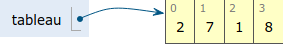
\includegraphics[width=0.5\textwidth,height=\textheight]{images/tableau0.png}\\

\hypertarget{tableaux-en-python}{%
\section{Tableaux en Python}\label{tableaux-en-python}}

\begin{cours}{}

\begin{itemize}
\tightlist
\item
  En
  \href{https://docs.python.org/3/tutorial/datastructures.html}{Python},
  les tableaux sont implémentés dans le type
  \passthrough{\lstinline!list!} et on les nomme souvent listes même si
  les listes désignent en général une autre structure de données. Le
  type \passthrough{\lstinline!list!} est suffisamment flexible pour
  représenter la structure de données tableau et d'autres comme les
  listes, piles, files \ldots{} \emph{Dans la suite de ce cours, on
  désigne par tableaux, les objets de type
  \passthrough{\lstinline!list!} du langage
  \href{https://docs.python.org/3/tutorial/datastructures.html}{Python}.
  Dans les exercices, comme dans les QCM d'E3C, on rencontrera parfois
  l'appellation Python liste pour désigner la structure de données
  tableau}
\item
  Un tableau
  \href{https://docs.python.org/3/tutorial/datastructures.html}{Python}
  est une expression délimitée par des crochets et les éléments dans
  l'ordre croissant des index de gauche à droite sont séparés par le
  symbole virgule \passthrough{\lstinline!,!} :
\end{itemize}

\begin{lstlisting}[language=Python]
  >>> t = [4, 20, 10] # on affecte le tableau [4, 20, 10] à t
  >>> len(t)
  3
  >>> t[0]
  4
  >>> t[len(t)-1]
  10
  >>> t[3]
  Traceback (most recent call last):
    File "<stdin>", line 1, in <module>
  IndexError: list index out of range   
  >>> t[0] = 6
  >>> t
  [6, 20, 10]
\end{lstlisting}

\begin{itemize}
\tightlist
\item
  La séquence de valeurs contenue dans un tableau est indexée à partir
  de 0.
\item
  Le \textbf{nombre d'éléments} d'un tableau affecté à une variable
  \passthrough{\lstinline!t!} est donné par la fonction
  \passthrough{\lstinline!len!} avec \passthrough{\lstinline!len(t)!}.
  Un \textbf{tableau vide} est noté \passthrough{\lstinline![]!}.
\item
  On accède à l'élément d'index \passthrough{\lstinline!k!} avec la
  syntaxe \passthrough{\lstinline!t[k]!}.
\item
  On peut manipuler l'élément d'index \passthrough{\lstinline!k!} comme
  une variable et modifier sa valeur par une affectation avec la syntaxe
  \passthrough{\lstinline!t[k] = valeur!}.
\item
  On peut considérer que l'accès et la modification d'un élément à
  partir de son index se fait en \textbf{temps constant}, car les
  éléments sont stockés de façon contigue en mémoire et l'index donne le
  nombre de décalages depuis le premier élément.
\item
  Un tableau est \textbf{itérable}, c'est-à-dire qu'on peut parcourir
  ses éléments avec une boucle \passthrough{\lstinline!for!}:\\
\end{itemize}

\begin{lstlisting}[language=Python]
>>> for e in t:
...     print(e)
... 
4
20
10
\end{lstlisting}

\begin{itemize}
\tightlist
\item
  En
  \href{https://docs.python.org/3/tutorial/datastructures.html}{Python},
  les tableaux peuvent contenir des éléments de types hétérogènes mais
  nous manipulerons principalement des tableaux homogènes (types
  \passthrough{\lstinline!int, float, string!},
  \passthrough{\lstinline!bool!}).
\item
  En
  \href{https://docs.python.org/3/tutorial/datastructures.html}{Python},
  les tableaux sont \textbf{dynamiques}, leur taille peut varier.
\end{itemize}

\end{cours}

\hypertarget{accuxe8s-aux-uxe9luxe9ments-dun-tableau}{%
\section{Accès aux éléments d'un
tableau}\label{accuxe8s-aux-uxe9luxe9ments-dun-tableau}}

\begin{methode}{}

\begin{itemize}
\tightlist
\item
  Dans un tableau \passthrough{\lstinline!tab!}, chaque élément de la
  séquence ordonnée est repéré par son index \passthrough{\lstinline!k!}
  qui permet d'accéder à l'élément avec l'expression
  \passthrough{\lstinline!tab[k]!} ou de le modifier avec l'instruction
  \passthrough{\lstinline!tab[k] = valeur!}.
\item
  \href{https://docs.python.org/3/tutorial/datastructures.html}{Python}
  permet également d'extraire un sous-tableau d'un tableau
  \passthrough{\lstinline!tab!} avec l'expression
  \passthrough{\lstinline!tab[debut:fin]!} qui représente la
  sous-séquence de \passthrough{\lstinline!fin - debut!} éléments, entre
  l'élément d'index \passthrough{\lstinline!debut!} inclus et l'élément
  d'index \passthrough{\lstinline!fin!} exclu, comme pour
  \passthrough{\lstinline!range(debut, fin)!}. Ce mécanisme de découpage
  en tranches est désigné par le terme de \emph{slicing}.
\item
  \href{https://docs.python.org/3/tutorial/datastructures.html}{Python}
  permet de repérer les éléments avec des index négatifs représentant le
  décalage par rapport à la la fin de la séquence, mais nous ne les
  utiliserons pas car ils sont source d'erreurs.
\end{itemize}

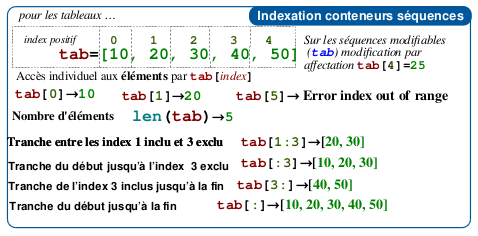
\includegraphics{images/slices.png}\\

\emph{Figure modifiée à partir d'une source de Louis Leskow inspirée
d'un memento de Laurent Pointal}

\begin{itemize}
\tightlist
\item
  On peut tester l'appartenance d'un élément à un tableau avec
  l'opérateur \passthrough{\lstinline!in!} et sa négation
  \passthrough{\lstinline!not in!}. Cette opération s'effectue en
  moyenne en coût proportionnel à la taille du tableau.
\end{itemize}

\begin{lstlisting}[language=Python]
>>> t = list(range(6))
>>> t
[0, 1, 2, 3, 4, 5]
>>> 4 in t
True
>>> 6 in t
False
>>> 6 not in t
True
\end{lstlisting}

\end{methode}

\begin{exercice}{}

\begin{enumerate}
\def\labelenumi{\arabic{enumi}.}
\tightlist
\item
  Soit la liste suivante :
  \passthrough{\lstinline!liste\_pays = ["France","Allemagne","Italie","Belgique"]!}.
\end{enumerate}

Que renvoie : \passthrough{\lstinline!liste\_pays[2]!} ?

\begin{enumerate}
\def\labelenumi{\arabic{enumi}.}
\setcounter{enumi}{1}
\tightlist
\item
  Quelle est la valeur référencée par le tableau L après exécution du
  programme ci-dessous ?
\end{enumerate}

\begin{lstlisting}[language=Python]
L = [731, 732, 734]
L[0], L[1] = L[1], L[0]
M = L
M[1] = 732
\end{lstlisting}

\textbf{Réponse 1 :} {[}732, 731, 734{]} \textbf{Réponse 2 :} {[}731,
732, 734{]} \textbf{Réponse 3 :} {[}732, 732, 734{]}

\begin{enumerate}
\def\labelenumi{\arabic{enumi}.}
\setcounter{enumi}{2}
\item
  On définit : \passthrough{\lstinline!L = [10,9,8,7,6,5,4,3,2,1]!}.
  Quelle est la valeur de \passthrough{\lstinline!L[L[3]]!} ?

  \begin{itemize}
  \tightlist
  \item
    \textbf{Réponse 1 :} 3 \textbf{Réponse 2 :} 4
  \item
    \textbf{Réponse 3 :} 7 \textbf{Réponse 4 :} 8
  \end{itemize}
\item
  Écrire une fonction \passthrough{\lstinline!recherche(tab, element)!}
  qui prend en paramètre un tableau et un élément et qui retourne
  \passthrough{\lstinline!True!} si \passthrough{\lstinline!element!}
  est dans \passthrough{\lstinline!tab!} et
  \passthrough{\lstinline!False!} sinon.
\end{enumerate}

\end{exercice}

\hypertarget{construction-dun-tableau}{%
\section{Construction d'un tableau}\label{construction-dun-tableau}}

\begin{methode}{}

Il existe plusieurs façons de définir un tableau en
\href{https://docs.python.org/3/tutorial/datastructures.html}{Python}.

\begin{itemize}
\tightlist
\item
  On peut le définir en \textbf{extension} en énumérant toute la
  séquence :
\end{itemize}

\begin{lstlisting}[language=Python]
>>> t1 = [8, 10, 11,14]
>>> t2 = [False, True, False]
\end{lstlisting}

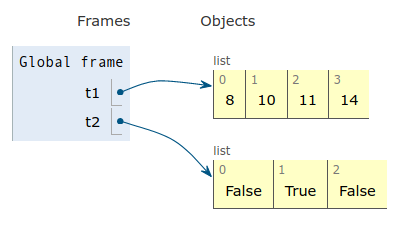
\includegraphics[width=0.5\textwidth,height=\textheight]{images/tableau1.png}\\

\begin{itemize}
\tightlist
\item
  On peut convertir en tableau un autre objet itérable (qui peut se
  parcourir avec une boucle \passthrough{\lstinline!for!}) avec le
  constructeur \passthrough{\lstinline!list!}.
\end{itemize}

\begin{lstlisting}[language=Python]
>>> t11 = list(range(5))
>>> t11
[0, 1, 2, 3, 4]
>>> t12 = list('alphabet')
>>> t12
['a', 'l', 'p', 'h', 'a', 'b', 'e', 't']
>>> list(4)
Traceback (most recent call last):
  File "<stdin>", line 1, in <module>
TypeError: 'int' object is not iterable
\end{lstlisting}

\begin{itemize}
\tightlist
\item
  On peut le définir en \textbf{compréhension} en générant ses éléments
  par une boucle \passthrough{\lstinline!for!} sur un itérable (
  générateur d'entiers \passthrough{\lstinline!range!}, autre tableau
  \ldots) combinée éventuellement avec un filtrage par une instruction
  conditionnelle :
\end{itemize}

\begin{lstlisting}[language=Python]
>>> t3 = [k ** 2 for k in range(6)]  #carrés des entiers entre 0 et 5
>>> t3
[0, 1, 4, 9, 16, 25]
>>> t4 = [k for k in range(len(t2)) if t2[k]]  # index des éléments de t2 de valeur True
>>> t4
[1]
\end{lstlisting}

\end{methode}

\begin{exercice}{}

\begin{enumerate}
\def\labelenumi{\arabic{enumi}.}
\item
  \emph{Auteur : Germain Becker, question n°326 Genumsi}.

  Quel est le tableau \passthrough{\lstinline!t!} construit par les
  instructions suivantes ?

\begin{lstlisting}[language=Python]
tab = [1, 2, -3, 7, 4, 10, -1, 0]
t = [e for e in tab if e >= 0]
\end{lstlisting}

  \begin{itemize}
  \tightlist
  \item
    \textbf{Réponse 1 :}
    \passthrough{\lstinline!t = [1, 2, 7, 4, 10, 0]!}
  \item
    \textbf{Réponse 2 :}
    \passthrough{\lstinline!t = [e, e, e, e, e, e]!}
  \item
    \textbf{Réponse 3 :} \passthrough{\lstinline!t = [1, 2, 7, 4, 10]!}
  \item
    \textbf{Réponse 4 :} \passthrough{\lstinline!t = [-3, -1, 0]!}
  \end{itemize}
\item
  Quel est le résultat de l'évaluation de l'expression Python suivante ?
  \emph{Auteur : Eric Rougier}

  \passthrough{\lstinline![2 ** n for n in range(4)]!}

  Réponses :

  \begin{itemize}
  \tightlist
  \item
    \textbf{Réponse 1 :} \passthrough{\lstinline![0, 2, 4, 6, 8]!}
  \item
    \textbf{Réponse 2 :} \passthrough{\lstinline![1, 2, 4, 8]!}
  \item
    \textbf{Réponse 3 :} \passthrough{\lstinline![0, 1, 4, 9]!}
  \item
    \textbf{Réponse 4 :} \passthrough{\lstinline![1, 2, 4, 8, 16]!}
  \end{itemize}
\item
  Qu'affiche le programme
  \href{https://docs.python.org/3/tutorial/datastructures.html}{Python}
  ci-dessous ?
\end{enumerate}

\begin{lstlisting}[language=Python]
L=[0,1,2]
M=[3,4,5]
N=[L[i]+M[i] for i in range(len(L))]
print(N)
\end{lstlisting}

\begin{enumerate}
\def\labelenumi{\arabic{enumi}.}
\setcounter{enumi}{3}
\item
  On exécute le script suivant :

\begin{lstlisting}[language=Python]
L = [12,0,8,7,3,1,5,3,8]

a = [elt for elt in L if elt < 4]
\end{lstlisting}

  Quelle est la valeur de \passthrough{\lstinline!a!} à la fin de son
  exécution ?

  \begin{itemize}
  \tightlist
  \item
    \textbf{Réponse 1 :} \passthrough{\lstinline![12,0,8]!}
    \textbf{Réponse 2 :} \passthrough{\lstinline![12,0,8,7]!}
  \item
    \textbf{Réponse 3 :} \passthrough{\lstinline![0,3,1,3]!}
    \textbf{Réponse 4 :} \passthrough{\lstinline![0,3,1]!}
  \end{itemize}
\end{enumerate}

\end{exercice}

\hypertarget{opuxe9rations-sur-les-tableaux}{%
\section{Opérations sur les
tableaux}\label{opuxe9rations-sur-les-tableaux}}

\begin{methode}{}

\begin{itemize}
\tightlist
\item
  On peut concaténer deux tableaux avec l'opérateur
  \passthrough{\lstinline!+!}, un nouveau tableau est renvoyé.
\end{itemize}

\begin{lstlisting}[language=Python]
>>> t1 = [1,2]
>>> t2 = [3,4]
>>> t3 = t1 + t2
>>> t3
[1, 2, 3, 4]
\end{lstlisting}

\begin{itemize}
\tightlist
\item
  L'opérateur \passthrough{\lstinline!*!} permet d'itérer une
  concaténation et d'initialiser un tableau de taille quelconque avec
  une valeur par défaut. Attention, c'est le même élément qui est
  dupliqué !
\end{itemize}

\begin{lstlisting}[language=Python]
>>> t0 = [0] * 4   #un tableau de taille 4 initialisé à 0
>>> t0
[0, 0, 0, 0]
>>> tv = [True] * 6  #un tableau de taille 6 initialisé à True
>>> tv
[True, True, True, True, True, True]
>>> from random import randint
>>> t1 = [randint(1, 6) for _ in range(5)]  #5 lancers de dé à 6 faces
>>> t1
[5, 2, 2, 5, 6]
>>> t2 = [randint(1, 6)] * 5 #5 lancers de dé à 6 faces ?
>>> t2                      #non 5 fois le même lancer
[5, 5, 5, 5, 5]
\end{lstlisting}

\end{methode}

\begin{exercice}{}

\begin{enumerate}
\def\labelenumi{\arabic{enumi}.}
\item
  On exécute le script suivant :

\begin{lstlisting}[language=Python]
a = [1, 2, 3]
b = [4, 5, 6]
c = a + b
\end{lstlisting}

  Que contient la variable \passthrough{\lstinline!c!} à la fin de cette
  exécution ?

  Réponses :

  \begin{itemize}
  \item
    \textbf{Réponse 1 :} \passthrough{\lstinline![5,7,9]!}
    \textbf{Réponse 2 :} \passthrough{\lstinline![1,4,2,5,3,6]!}
  \item
    \textbf{Réponse 3 :} \passthrough{\lstinline![1,2,3,4,5,6]!}
    \textbf{Réponse 4 :} \passthrough{\lstinline![1,2,3,5,7,9]!}
  \end{itemize}
\item
  Soit la fonction \passthrough{\lstinline!mystere!} ci-dessous.

  Quelle est la valeur retournée par
  \passthrough{\lstinline!mystere([831, 832, 833, 841, 842, 843])!} ?

\begin{lstlisting}[language=Python]
def mystere(u):
  v = []
  n = len(u)
  for k in range(n):
    v = [u[k]]+v
  return v
\end{lstlisting}
\end{enumerate}

\end{exercice}

\hypertarget{parcours-dun-tableau}{%
\section{Parcours d'un tableau}\label{parcours-dun-tableau}}

\begin{methode}{}

Il existe deux façons de parcourir un tableau en
\href{https://docs.python.org/3/tutorial/datastructures.html}{Python} :

\begin{enumerate}
\def\labelenumi{\arabic{enumi}.}
\tightlist
\item
  \textbf{Le parcours par élément}, puisqu'un tableau de type
  \passthrough{\lstinline!list!} est \textbf{itérable} en
  \href{https://docs.python.org/3/tutorial/datastructures.html}{Python}
  :
\end{enumerate}

\begin{lstlisting}[language=Python]
>>> t6 = [3, 1, 4]
>>> for e in t6:
...     print("valeur : ", e)
... 
valeur :  3
valeur :  1
valeur :  4
\end{lstlisting}

\begin{enumerate}
\def\labelenumi{\arabic{enumi}.}
\setcounter{enumi}{1}
\tightlist
\item
  \textbf{Le parcours par index}, permet de récupérer les indexs des
  éléments en plus de leurs valeurs :
\end{enumerate}

\begin{lstlisting}[language=Python]
>>> for k in range(len(t6)):
...     print("valeur : ", t6[k], " index :", k)
... 
valeur :  3  index : 0
valeur :  1  index : 1
valeur :  4  index : 2
\end{lstlisting}

\end{methode}

\begin{exercice}{}

\begin{enumerate}
\def\labelenumi{\arabic{enumi}.}
\item
  Écrire une fonction \passthrough{\lstinline!occurences(v, t)!} qui
  retourne le nombre d'occurences de la valeur
  \passthrough{\lstinline!v!} dans le tableau
  \passthrough{\lstinline!t!}.
\item
  \emph{Auteur : Nicolas Réveret, question n°379 Genumsi}

  On a saisi le code suivant :

\begin{lstlisting}[language=Python]
liste = [0, 1, 2, 3]
compteur = 0
for i in range(len(liste)-1) :
    for j in range(i,len(liste)) :
        compteur += 1
\end{lstlisting}

  Que contient la variable compteur à la fin de l'exécution de ce script
  ?
\item
  Revenons sur notre situation d'accroche.
\end{enumerate}

\begin{itemize}
\tightlist
\item
  Écrire une fonction \passthrough{\lstinline!somme(tab)!} qui retourne
  la somme des éléments d'un tableau de nombres
  \passthrough{\lstinline!tab!}.
\item
  Écrire une fonction
  \passthrough{\lstinline!moyenne\_arithmetique(tab)!} qui retourne la
  moyenne arithmétique des éléments d'un tableau de nombres
  \passthrough{\lstinline!tab!}.
\end{itemize}

\begin{enumerate}
\def\labelenumi{\arabic{enumi}.}
\setcounter{enumi}{3}
\item
  En voulant programmer une fonction qui calcule la valeur minimale d'un
  tableau d'entiers, on a écrit :

\begin{lstlisting}[language=Python]
def minimum(L):
    mini = 0
    for e in L:
        if e < mini:
            mini = e
    return mini
\end{lstlisting}

  Cette fonction a été mal programmée. Pour quel tableau ne
  donnera-t-elle pas le résultat attendu, c'est-à-dire son minimum ?

  Réponses :

  \begin{itemize}
  \tightlist
  \item
    \textbf{Réponse 1 :} \passthrough{\lstinline![-1,-8,12,2,23]!}
  \item
    \textbf{Réponse 2:} \passthrough{\lstinline![0,18,12,2,3]!}
  \item
    \textbf{Réponse 3:} \passthrough{\lstinline![-1,-1,12,12,23]!}
  \item
    \textbf{Réponse 4:} \passthrough{\lstinline![1,8,12,2,23]!}
  \end{itemize}
\item
  Écrire une fonction \passthrough{\lstinline!max\_tab(tab)!} qui
  retourne le maximum d'un tableau de nombres passé en paramètre.
\end{enumerate}

\end{exercice}

\hypertarget{aliasing}{%
\section{Aliasing}\label{aliasing}}

\hypertarget{aliasing-et-copie-de-tableau}{%
\subsection{Aliasing et copie de
tableau}\label{aliasing-et-copie-de-tableau}}

\begin{cours}{}

\begin{itemize}
\item
  Pour les tableaux (type \passthrough{\lstinline!list!}), comme pour
  les autres types construits, le mécanisme de l'affectation de variable
  en
  \href{https://docs.python.org/3/tutorial/datastructures.html}{Python}
  diffère de celui des types base :
  \passthrough{\lstinline!int, float, bool!}). Lors de l'affectation
  \passthrough{\lstinline!tab = [6, 3, 1]!}, la variable
  \passthrough{\lstinline!tab!} ne reçoit pas comme valeur les éléments
  du tableau mais une \textbf{référence} vers la zone mémoire où ils
  sont effectivement stockés. Ce mécanisme est désigné par le terme
  \emph{d'aliasing}.
\item
  Illustrons ces différences en déroulant une séquence d'affectations
  avec
  \href{http://pythontutor.com/visualize.html\#mode=edit}{Python-tutor},
  où l'on copie par affectation une variable de type
  \passthrough{\lstinline!int!} puis une variable de type
  \passthrough{\lstinline!list!}.

  \begin{itemize}
  \tightlist
  \item
    \textbf{Étape 1 :} Si \passthrough{\lstinline!a!} est de type de
    base (ici \passthrough{\lstinline!int!}), l'affectation
    \passthrough{\lstinline!b = a!} assigne à la variable
    \passthrough{\lstinline!b!} une copie de la valeur de la variable
    \passthrough{\lstinline!a!} (ici 50.)
  \end{itemize}

  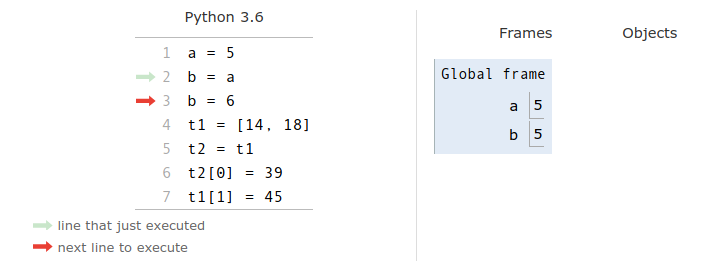
\includegraphics{images/aliasing1.png}\\

  \begin{itemize}
  \tightlist
  \item
    \textbf{Étape 2 :} Si on modifie la valeur de
    \passthrough{\lstinline!b!}, la variable \passthrough{\lstinline!a!}
    n'est pas touchée, les deux variables sont indépendantes.
  \end{itemize}

  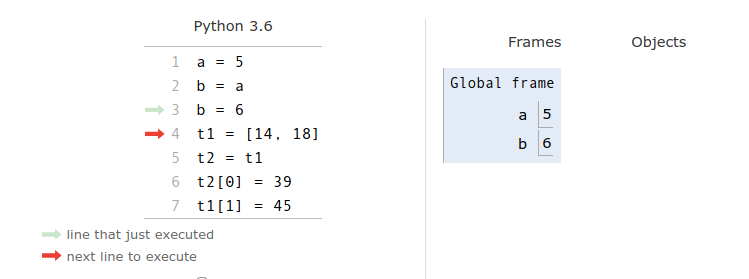
\includegraphics{images/aliasing2.png}\\

  \begin{itemize}
  \tightlist
  \item
    \textbf{Étape 3 :} Si on affecte le tableau
    \passthrough{\lstinline![14, 18]!} à la variable
    \passthrough{\lstinline!t1!}, celle-ci ne prend pas pour valeur
    directement la séquence d'éléments du tableau mais une
    \textbf{référence} vers cette séquence.
  \end{itemize}

  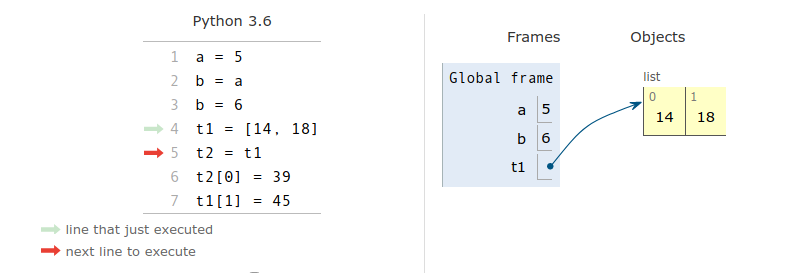
\includegraphics{images/aliasing3.png}\\

  \begin{itemize}
  \item
    \textbf{Étape 4 :} Si \passthrough{\lstinline!t1!} est de type
    construit (ici \passthrough{\lstinline!list!}), l'affectation
    \passthrough{\lstinline!t2 = t1!} assigne à la variable
    \passthrough{\lstinline!t2!} une copie de la valeur de la variable
    \passthrough{\lstinline!t1!} comme pour les types de base, sauf que
    la valeur de \passthrough{\lstinline!t1!} est une
    \textbf{référence}. On dit que \passthrough{\lstinline!t1!} et
    \passthrough{\lstinline!t2!} partagent la même référence.

    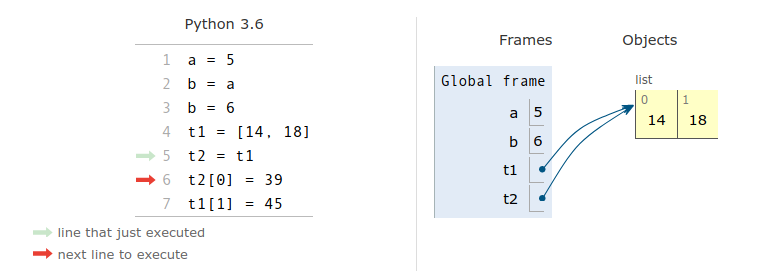
\includegraphics{images/aliasing4.png}\\
  \item
    \textbf{Étape 5 :} Comme \passthrough{\lstinline!t1!} et
    \passthrough{\lstinline!t2!} partagent la même référence, toute
    modification de \passthrough{\lstinline!t1!} touche
    \passthrough{\lstinline!t2!} et vice-versa. On parle \textbf{d'effet
    de bord}. Attention, il faut bien comprendre ce mécanisme pour
    éviter les effets de bord indésirables !

    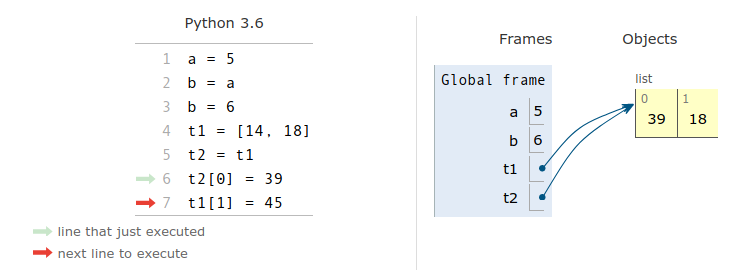
\includegraphics{images/aliasing5.png}\\

    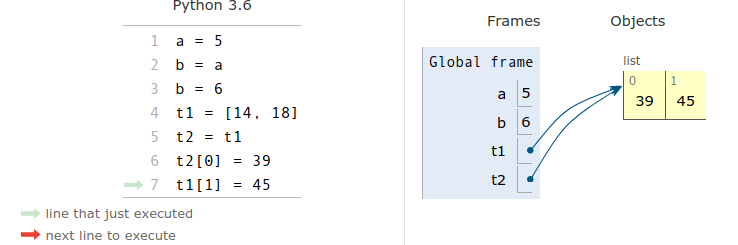
\includegraphics{images/aliasing6.png}\\
  \end{itemize}
\item
  On peut réaliser une \textbf{copie superficielle} (ou \emph{shallow
  copy}) d'un tableau ou d'une variable de type construit avec le
  mécanisme de \emph{slicing}. Noys y reviendrons plus tard, pour les
  structures imbriquées (tableaux de tableaux), il faudra copier
  récursivement les valeurs correspondant à toutes les références avec
  une \textbf{copie profonde}. Le module \passthrough{\lstinline!copy!}
  propose une fonction \passthrough{\lstinline!copy!} pour la copy
  superficielle et une fonction \passthrough{\lstinline!deepcopy!} pour
  la copie profonde.

  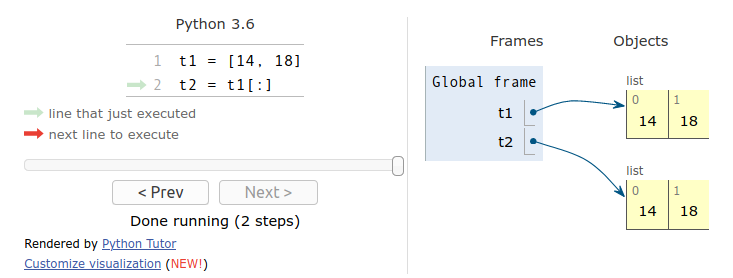
\includegraphics{images/shallow-copy.png}\\
\end{itemize}

\end{cours}

\begin{exercice}{}

\begin{enumerate}
\def\labelenumi{\arabic{enumi}.}
\item
  Écrire une fonction \passthrough{\lstinline!copie(tab)!} qui retourne
  une copie superficielle du tableau \passthrough{\lstinline!tab!} sans
  utiliser de \emph{slicing}.
\item
  \emph{Auteur : Nicolas Revéret}

  On considère le code suivant :

\begin{lstlisting}[language=Python]
def f(tab):
  for i in range(len(tab)//2):
    tab[i],tab[-i-1] = tab[-i-1],tab[i]
\end{lstlisting}

  Après les lignes suivantes :

\begin{lstlisting}[language=Python]
tab = [2,3,4,5,7,8]
f(tab)
\end{lstlisting}

  Quelle est la valeur de la variable \passthrough{\lstinline!tab!} ?

  Réponses :

  \begin{itemize}
  \tightlist
  \item
    \textbf{Réponse 1} \passthrough{\lstinline![2,3,4,5,7,8]!}
    \textbf{Réponse 2} \passthrough{\lstinline![5,7,8,2,3,4]!}
  \item
    \textbf{Réponse 3} \passthrough{\lstinline![8,7,5,4,3,2]!}
    \textbf{Réponse 4} \passthrough{\lstinline![4,3,2,8,7,5]!}
  \end{itemize}
\end{enumerate}

\end{exercice}

\hypertarget{aliasing-et-passage-de-tableau-en-paramuxe8tre-dune-fonction}{%
\subsection{Aliasing et passage de tableau en paramètre d'une
fonction}\label{aliasing-et-passage-de-tableau-en-paramuxe8tre-dune-fonction}}

\begin{methode}{}

En
\href{https://docs.python.org/3/tutorial/datastructures.html}{Python},
lorsqu'on appelle une fonction avec des \textbf{paramètres effectifs},
les \textbf{paramètres formels} apparaissant dans la signature de la
fonction, deviennent des variables locales à la fonction et reçoivent
comme valeurs des copies des valeurs des paramètres effectifs. Les types
construits, comme les tableaux de type \passthrough{\lstinline!list!},
ayant pour valeur une référence, le paramètre formel va partager la même
référence et on va retrouver les mêmes effets de bord que dans la copie
de tableau par affectation.

\begin{itemize}
\item
  \textbf{Étape 1 :} On définit une variable globale
  \passthrough{\lstinline!a!} de type \passthrough{\lstinline!int!}, une
  variable \passthrough{\lstinline!t1!} de type
  \passthrough{\lstinline!list!} (un tableau), une fonction
  \passthrough{\lstinline!incremente(x)!} qui incrémente la valeur du
  paramètre \passthrough{\lstinline!x!} de type
  \passthrough{\lstinline!int!} et une fonction
  \passthrough{\lstinline!incremente\_tab(tab)!} qui incrémente tous les
  éléments du paramètre \passthrough{\lstinline!tab!}de type
  \passthrough{\lstinline!list!}.

  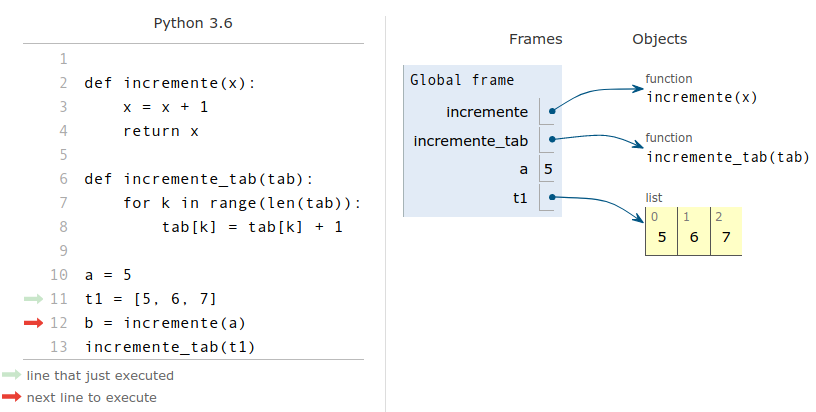
\includegraphics{images/aliasing-fonction1.png}\\
\item
  \textbf{Étape 2 :} On appelle \passthrough{\lstinline!incremente(a)!}
  et on affecte la valeur retournée à une variable
  \passthrough{\lstinline!b!}. Lors de l'appel, le paramètre formel
  \passthrough{\lstinline!x!} prend pour valeur une copie de la valeur
  du paramètre effectif \passthrough{\lstinline!a!}. La fonction
  retourne la valeur 6 après incrémentation de la variable
  \passthrough{\lstinline!x!}, les variables globale
  \passthrough{\lstinline!a!} et locale \passthrough{\lstinline!x!} sont
  indépendantes. \passthrough{\lstinline!x!} disparaît dès que l'appel
  de fonction se termine.

  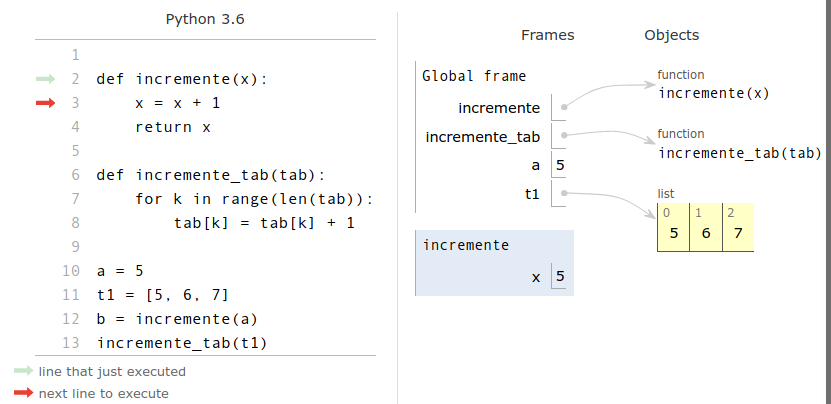
\includegraphics{images/aliasing-fonction2.png}\\

  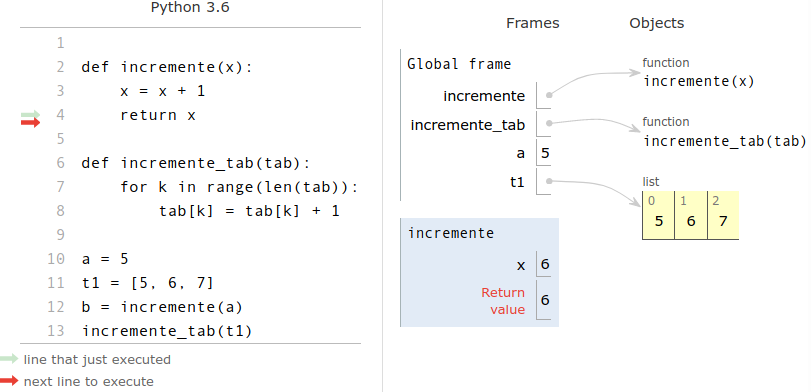
\includegraphics{images/aliasing-fonction25.png}\\
\item
  \textbf{Étape 3 :} La variable globale \passthrough{\lstinline!b!} a
  été affectée avec 6 la valeur retournée par
  \passthrough{\lstinline!incremente(a)!}. La variable
  \passthrough{\lstinline!a!} n'a pas été modifiée par effet de bord,.
  Lors de l'appel \passthrough{\lstinline!incremente\_tab(t1)!}, le
  paramètre formel \passthrough{\lstinline!tab!} est affecté avec une
  copie de la valeur du paramètre effectif \passthrough{\lstinline!t1!}.
  Ce dernier n'est pas de type de base comme
  \passthrough{\lstinline!a!}, mais de type construit
  \passthrough{\lstinline!list!} donc sa valeur est un référence.

  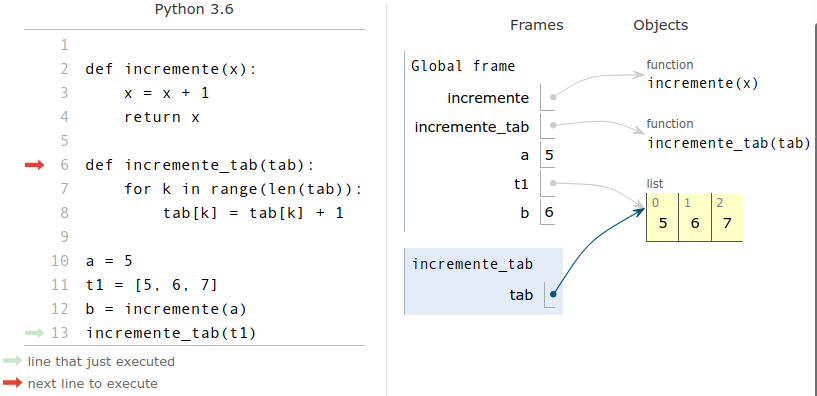
\includegraphics{images/aliasing-fonction3.png}\\
\item
  \textbf{Étape 4 :} La variable locale \passthrough{\lstinline!tab!} et
  la variable globale \passthrough{\lstinline!t1!} partagent une même
  référence : la fonction \passthrough{\lstinline!incremente\_tab!} peut
  modifier le tableau référencé . La fonction
  \passthrough{\lstinline!incremente\_tab!} renvoie
  \passthrough{\lstinline!None!} même si elle ne contient pas
  d'instruction \passthrough{\lstinline!return!}. Après l'appel de
  fonction, la variable globale \passthrough{\lstinline!t1!} a été
  modifiée par par \textbf{effet de bord}. Une fonction qui modifie
  l'état de la mémoire du programme principale, sans renvoyer de valeur,
  s'appelle une \textbf{procédure}.

  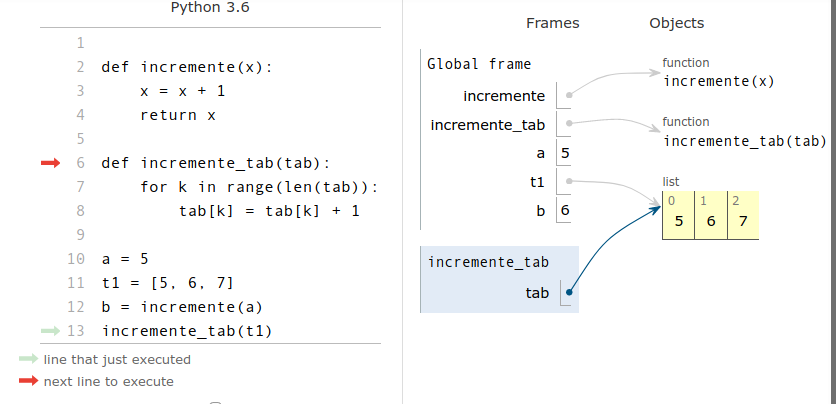
\includegraphics{images/aliasing-fonction4.png}\\

  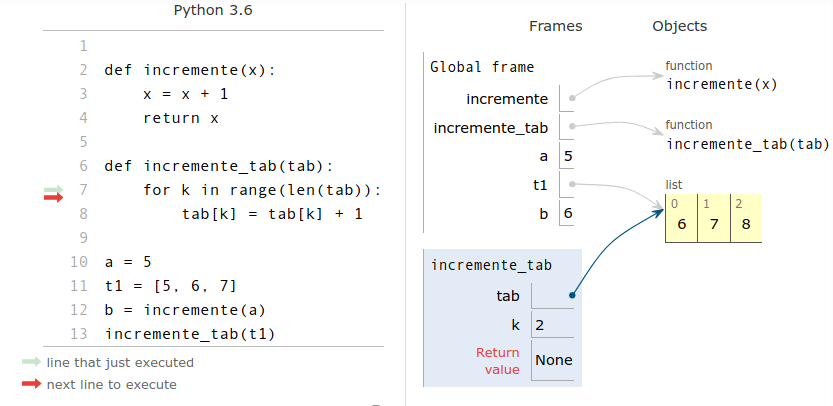
\includegraphics{images/aliasing-fonction5.png}\\

  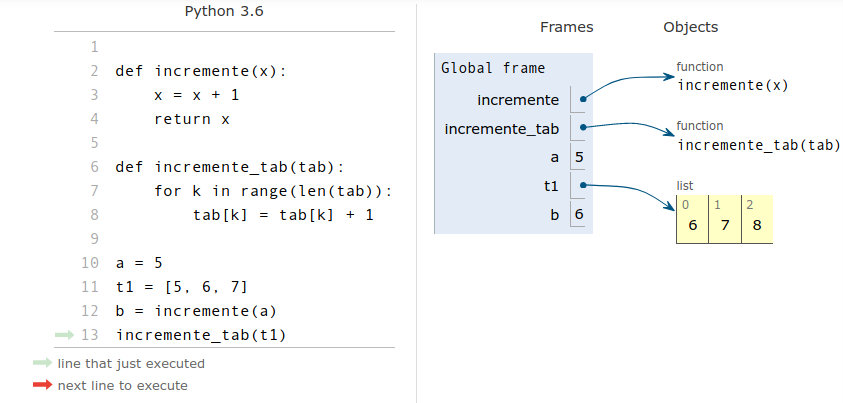
\includegraphics{images/aliasing-fonction6.png}\\
\end{itemize}

\end{methode}

\begin{exercice}{}

\begin{enumerate}
\def\labelenumi{\arabic{enumi}.}
\item
  On veut écrire une procédure
  \passthrough{\lstinline!echange(tab, i, j)!} qui échange les éléments
  d'index \passthrough{\lstinline!i!} et \passthrough{\lstinline!j!}
  d'un tableau \passthrough{\lstinline!tab!}. On fournit le modèle
  ci-dessous :

\begin{lstlisting}[language=Python]
def echange(tab, i, j):
  assert 0 <= i < len(tab) and 0 <= j < len(tab), "message d'erreur"
  # à compléter
\end{lstlisting}

  \begin{itemize}
  \tightlist
  \item
    Remplacer le message d'erreur de l'assertion par un message
    pertinent.
  \item
    Compléter la fonction.
  \end{itemize}
\item
  Écrire une procédure
  \passthrough{\lstinline!permutation\_circulaire(tab)!} qui modifie la
  position des éléments du tableau \passthrough{\lstinline!tab!} par
  permutation circulaire de gauche à droite :\\
\end{enumerate}

\begin{lstlisting}[language=Python]
>>> t = list(range(6))
>>> t
[0, 1, 2, 3, 4, 5]
>>> permutation_circulaire(t)
>>> t
[5, 0, 1, 2, 3, 4]
>>> permutation_circulaire(t)
>>> t
[4, 5, 0, 1, 2, 3]
\end{lstlisting}

\end{exercice}

\hypertarget{muxe9thodes-de-tableau-dynamique-en-python}{%
\section{Méthodes de tableau dynamique en
Python}\label{muxe9thodes-de-tableau-dynamique-en-python}}

\begin{methode}{}

Les tableaux
\href{https://docs.python.org/3/tutorial/datastructures.html}{Python}
sont dynamiques c'est-à-dire que leur taille peut évoluer. Pour un
tableau \passthrough{\lstinline!tab!}, les fonctions permettant
d'ajouter ou enlever des éléments sont des \textbf{méthodes} de l'objet
\passthrough{\lstinline!tab!} qui s'utilisent avec la notation pointée
\passthrough{\lstinline!tab.methode(parametres)!}. Un tableau étant de
type \passthrough{\lstinline!list!} il est équivalent d'écrire
\passthrough{\lstinline!list.methode(tab, parametres)!}.

\begin{lstlisting}[language=Python]
>>> t = []   #tableau vide
>>> t.append(8)  #ajout de l'élément 8 à la fin de t
>>> t
[8]
>>> list.append(t, 7)  #ajout de l'élément 7 à la fin de t
>>> t
[8, 7]
\end{lstlisting}

\begin{itemize}
\tightlist
\item
  On peut ajouter un élément à la fin d'un tableau avec la méthode
  \passthrough{\lstinline!append!}. On peut ainsi peupler un tableau
  initialement vide.
\end{itemize}

\begin{lstlisting}[language=Python]
>>> t5 = []
>>> for k in range(3):
...     t5 .append(k ** 2)
... 
>>> t5
[0, 1, 4]
\end{lstlisting}

\begin{itemize}
\tightlist
\item
  On peut insérer un élément avec la méthode
  \passthrough{\lstinline!insert!} qui prend en paramètre l'index de
  l'élément une fois inséré. Les éléments à sa droite étant tous décalés
  vers la droite, l'insertion peut représenter un coût proportionnel à
  la taille du tableau si elle se fait au début du tableau.
\end{itemize}

\begin{lstlisting}[language=Python]
>>> t = ['a', 'c', 'd']
>>> t.insert(1, 'b')
>>> t
['a', 'b', 'c', 'd']
\end{lstlisting}

\begin{itemize}
\item
  On peut extraire un élément de deux façons :

  \begin{itemize}
  \tightlist
  \item
    À partir de son index, avec la méthode
    \passthrough{\lstinline!pop!}, qui prend pour paramètre l'index de
    l'élément extrait, le dernier par défaut. Tous les éléments à droite
    de l'élément extrait doivent être décalés vers la gauche, ce qui
    peut représenter un coût proportionnel à la taille du tableau si
    l'extraction se fait au début du tableau.
  \end{itemize}

\begin{lstlisting}[language=Python]
>>> carac = [chr(k) for k in range(ord('a'), ord('g'))]
>>> carac
['a', 'b', 'c', 'd', 'e', 'f']
>>> carac.pop()
'f'
>>> carac
['a', 'b', 'c', 'd', 'e']
>>> carac.pop(0)
'a'
>>> carac
['b', 'c', 'd', 'e']
\end{lstlisting}

  \begin{itemize}
  \tightlist
  \item
    À partir de sa valeur avec la méthode
    \passthrough{\lstinline!remove!}, la première occurence trouvée de
    l'élément passée en paramètre est supprimée. Encore une fois, le
    coût peut être proportionnel à la taille du tableau si la
    suppression se fait au début.
  \end{itemize}

\begin{lstlisting}[language=Python]
>>> t = [0,1,0,1]
>>> t = [0,2,0,2]
>>> t.remove(2)
>>> t
[0, 0, 2]
>>> t.remove(1)
Traceback (most recent call last):
  File "<stdin>", line 1, in <module>
ValueError: list.remove(x): x not in list
\end{lstlisting}
\item
  On peut compter le nombre d'occurences d'un élément dans un tableau
  avec la méthode \passthrough{\lstinline!count!}.
\end{itemize}

\begin{lstlisting}[language=Python]
>>> t = [randint(1, 6) for _ in range(1_000_000)]  #10**6 lancers de dés 
>>> t.count(6)  #nombre de 6, cohérent non ?
166821
\end{lstlisting}

\end{methode}

\begin{exercice}{}

\begin{enumerate}
\def\labelenumi{\arabic{enumi}.}
\item
  Écrire une fonction fonction
  \passthrough{\lstinline!filtre\_notes(tab)!} qui extrait toutes les
  notes inférieures à 10 d'un tableau de notes entre 0 et 20 et les
  renvoie dans un autre tableau.
\item
  Écrire une fonction renvoyant le maximum d'un tableau passé en
  paramètre et le tableau des positions où ce maximum est atteint.
\item
  On définit en Python la fonction suivante :

\begin{lstlisting}[language=Python]
def f(L):
    S = []
    for i in range(len(L)-1):
        S.append(L[i] + L[i+1])
    return S
\end{lstlisting}

  Quel est le tableau renvoyé par
  \passthrough{\lstinline!f([1, 2, 3, 4, 5, 6])!}~?

  \begin{itemize}
  \tightlist
  \item
    \textbf{Réponse 1} \passthrough{\lstinline![3, 5, 7, 9, 11, 13]!}
  \item
    \textbf{Réponse 2} \passthrough{\lstinline![1, 3, 5, 7, 9, 11]!}
  \item
    \textbf{Réponse 3} \passthrough{\lstinline![3, 5, 7, 9, 11]!}
  \item
    \textbf{Réponse 4} cet appel de fonction déclenche un message
    d'erreur
  \end{itemize}
\end{enumerate}

\end{exercice}

\end{document}
